\documentclass[../main.tex]{subfiles}
\begin{document}

	\chapter{Approximation of functions}
	\label{chap:chap_2}
	Let $V$ be a function space spanned by a set of \textit{basis functions} $\psi_{0}, \ldots, \psi_{N}$,
	$$
	V=\operatorname{span}\left\{\psi_{0}, \ldots, \psi_{N}\right\},
	$$
	such that any function $u \in V$ can be written as a linear combination of the basis functions:
	\begin{equation}\label{eqa23}
		u=\sum_{j \in \mathcal{I}_{s}} c_{j} \psi_{j}.
	\end{equation}
	The index set $\mathcal{I}_{s}$ is defined as $\mathcal{I}_{s}=\{0, \ldots, N\}$ and is used both for compact notation and for flexibility in the numbering of elements in sequences.
	
	For now, in this introduction, we shall look at functions of a single variable $x: u=u(x), \psi_{i}=\psi_{i}(x), i \in \mathcal{I}_{s}$. Later, we will almost trivially extend the mathematical details to functions of two- or three-dimensional physical spaces.
	The approximation (\hyperref[eqa23]{23}) is typically used to discretize a problem in space. Other
	methods, most notably finite differences, are common for time discretization,
	although the form (\hyperref[eqa23]{23}) can be used in time as well.
	\section[The least squares method]{The least squares method}
	\label{sec:sec_2_1}
	
	\noindent Given a function $f(x)$, how can we determine its best approximation $u(x) \in V$ ? A natural starting point is to apply the same reasoning as we did for vectors in Section \hyperref[sec:sec_1_2]{1.2}. That is, we minimize the distance between $u$ and $f$. However, this requires a norm for measuring distances, and a norm is most conveniently defined through an inner product. Viewing a function as a vector of infinitely many point values, one for each value of $x$, the inner product could intuitively be defined as the usual summation of pairwise components, with summation replaced by integration:
	$$
	(f, g)=\int f(x) g(x) \mathrm{d} x.
	$$
	To fix the integration domain, we let $f(x)$ and $\psi_{i}(x)$ be defined for a domain $\Omega \subset \mathbb{R}$. The inner product of two functions $f(x)$ and $g(x)$ is then
	\begin{equation}\label{eqa24}
		(f, g)=\int_{\Omega} f(x) g(x) \mathrm{d} x.	
	\end{equation}
	The distance between $f$ and any function $u \in V$ is simply $f-u$, and the squared norm of this distance is
	\begin{equation}\label{eqa25}
		E=\left(f(x)-\sum_{j \in \mathcal{I}_{s}} c_{j} \psi_{j}(x), f(x)-\sum_{j \in \mathcal{I}_{s}} c_{j} \psi_{j}(x)\right).	
	\end{equation}
	
	\noindent Note the analogy with (\hyperref[eqa14]{14}) : the given function $f$ plays the role of the given vector $\boldsymbol{f}$, and the basis function $\psi_{i}$ plays the role of the basis vector $\psi_{i}$. We can rewrite (\hyperref[eqa25]{25}), through similar steps as used for the result (\hyperref[eqa14]{14}), leading to 
	\begin{equation}\label{eqa26}
		E\left(c_{i}, \ldots, c_{N}\right)=(f, f)-2 \sum_{j \in \mathcal{I}_{s}} c_{j}\left(f, \psi_{i}\right)+\sum_{p \in \mathcal{I}_{s}} \sum_{q \in \mathcal{I}_{s}} c_{p} c_{q}\left(\psi_{p}, \psi_{q}\right).	
	\end{equation}
	Minimizing this function of $N+1$ scalar variables $\left\{c_{i}\right\}_{i \subset \mathcal{I}_{\mathrm{s}}}$, requires differentiation with respect to $c_{i}$, for all $i \in \mathcal{I}_{8}$. The resulting cquations are very similar to those we had in the vector case, and we hence end up with a linear system of the form (\hyperref[eqa18]{18}), with basically the same expressions:
	\begin{equation}\label{eqa27}
		A_{i, j} \left(\psi_{i}, \psi_{j}\right),
	\end{equation}
	\begin{equation}\label{eqa28}
		b_{i} \left(f, \psi_{i}\right).
	\end{equation}
	\section[The projection (or Galerkin) method]{The projection (or Galerkin) method}
	\label{sec:sec_2_2}
	As in Section \hyperref[sec:sec_1_2]{1.2}, the minimization of $(e, e)$ is equivalent to
	\begin{equation}\label{eqa29}
		(e, v)=0, \quad \forall v \in V.
	\end{equation}
	This is known as a projection of a function $f$ onto the subspace $V$. We may also call it a Galerkin method for approximating functions. Using the same reasoning as in (\hyperref[eqa21]{21})-(\hyperref[eqa22]{22}), it follows that (\hyperref[eqa29]{29}) is equivalent to
	\begin{equation}\label{eqa30}
		\left(e, \psi_{i}\right)=0, \quad i \in \mathcal{I}_{s}.
	\end{equation}
	Inserting $e=f-u$ in this equation and ordering terms, as in the multidimensional vector case, we end up with a linear system with a coefficient matrix (\hyperref[eqa27]{27}) and right-hand side vector (\hyperref[eqa28]{28}).
	
	Whether we work with vectors in the plane, general vectors, or functions in function spaces, the least squares principle and the projection or Galerkin method are equivalent.
	
	\section[Example: linear approximation]{Example: linear approximation}
	\label{sec:sec_2_3}
	\noindent Let us apply the theory in the previous section to a simple problem: given a parabola $f(x)=10(x-1)^{2}-1$ for $x \in \Omega=[1,2]$, find the best approximation $u(x)$ in the space of all linear functions:
	$$
	V=\operatorname{span}\{1, x\} .
	$$
	With our notation, $\psi_{0}(x)=1, \psi_{1}(x)=x$, and $N=1$. We seek
	$$
	u=c_{0} \psi_{0}(x)+c_{1} \psi_{1}(x)=c_{0}+c_{1} x,
	$$
	where $c_{0}$ and $c_{1}$ are found by solving a $2 \times 2$ the linear system. The coefficient matrix has elements
	\begin{equation}\label{eqa31}
		A_{0,0}=\left(\psi_{0}, \psi_{0}\right)=\int_{1}^{2} 1 \cdot 1 \mathrm{~d} x=1,
	\end{equation}
	\begin{equation}\label{eqa32}
		A_{0,1}=\left(\psi_{0}, \psi_{1}\right)=\int_{1}^{2} 1 \cdot x \mathrm{~d} x=3/2,
	\end{equation}
	\begin{equation}\label{eqa33}
		A_{1,0}=A_{0,1}=3 / 2,
	\end{equation}
	\begin{equation}\label{eqa34}
		A_{1,1}=\left(\psi_{1}, \psi_{1}\right)=\int_{1}^{2} x \cdot x \mathrm{~d} x=7 / 3.
	\end{equation}
	The corresponding right-hand side is
	\begin{equation}\label{eqa35}
		b_{1}=\left(f, \psi_{0}\right)=\int_{1}^{2}\left(10(x-1)^{2}-1\right) \cdot 1 \mathrm{~d} x=7 / 3,
	\end{equation}
	\begin{equation}\label{eqa36}
		b_{2}=\left(f, \psi_{1}\right)=\int_{1}^{2}\left(10(x-1)^{2}-1\right) \cdot x \mathrm{~d} x=13 / 3.
	\end{equation}
	Solving the linear system results in
	\begin{equation}\label{eqa37}
		c_{0}=-38 / 3, \quad c_{1}=10,
	\end{equation}
	and consequently
	\begin{equation}\label{eqa38}
		u(x)=10 x-\frac{38}{3}.
	\end{equation}
	Figure \hyperref[fig:img_3]{3} displays the parabola and its best approximation in the space of all linear functions.
	\begin{figure}[H]
		\centering
		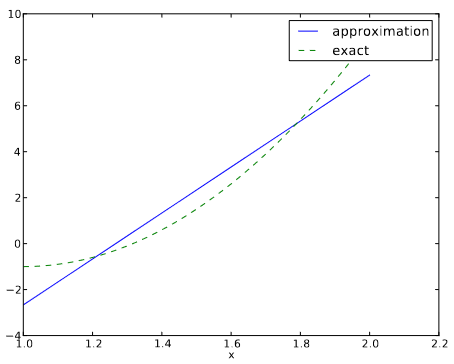
\includegraphics[width=0.7\linewidth]{img_3}
		\caption{Best approximation of a parabola by a straight line.}
		\label{fig:img_3}
	\end{figure}
	\section[Implementation of the least squares method]{Implementation of the least squares method}
	\label{sec:sec_2_4}
	\noindent The linear system can be computed either symbolically or numerically (a numer-
	ical integration rule is needed in the latter case). Here is a function for symbolic
	computation of the linear system, where f (x) is given as a sympy expression f
	involving the symbol x, psi is a list of expressions for $\left\{\psi_{i}\right\}_{i \in \mathcal{I}_{s}}$, and Omega is a 2-tuple/list holding the limits of the domain $\Omega$ :
	
	\begin{lstlisting}[numbers=none]
		import sympy as sp
		def least_squares(f, psi, Omega):
		N = len(psi) - 1
		A = sp.zeros((N+1, N+1))
		b = sp.zeros((N+1, 1))
		x = sp.Symbol('x')
		for i in range(N+1):
		for j in range(i, N+1):
		A[i,j] = sp.integrate(psi[i]*psi[j],
		(x, Omega[0], Omega[1]))
		A[j,i] = A[i,j]
		b[i,0] = sp.integrate(psi[i]*f, (x, Omega[0], Omega[1]))
		c = A.LUsolve(b)
		u = 0
		for i in range(len(psi)):
		u += c[i,0]*psi[i]
		return u, c
	\end{lstlisting}
	Observe that we exploit the symmetry of the coefficient matrix: only the
	upper triangular part is computed. Symbolic integration in sympy is often
	time consuming, and (roughly) halving the work has noticeable effect on the
	waiting time for the function to finish execution.
	
	Comparing the given f (x) and the approximate u(x) visually is done by
	the following function, which with the aid of sympy's lambdify tool converts a
	sympy expression to a Python function for numerical computations:
	\begin{lstlisting}[numbers=none]
		def comparison_plot(f, u, Omega, filename='tmp.pdf'):
		x = sp.Symbol('x')
		f = sp.lambdify([x], f, modules="numpy")
		u = sp.lambdify([x], u, modules="numpy")
		resolution = 401 # no of points in plot
		xcoor = linspace(Omega[0], Omega[1], resolution)
		exact = f(xcoor)
		approx = u(xcoor)
		plot(xcoor, approx)
		hold('on')
		plot(xcoor, exact)
		legend(['approximation', 'exact'])
		savefig(filename)
	\end{lstlisting}
	The modules='numpy' argument to lambdify is important if there are mathe-
	matical functions, such as sin or exp in the symbolic expressions in f or u, and
	these mathematical functions are to be used with vector arguments, like xcoor
	above.
	
	Both the least\textunderscore squares and comparison\textunderscore plot are found and coded in the
	file \href{http://tinyurl.com/jvzzcfn/fem/approx1D.py}{approx1D.py.} The forthcoming examples on their use appear in ex\textunderscore approx1D.py.
	\section[Perfect approximation]{Perfect approximation}
	\label{sec:sec_2_5}
	Let us use the code above to recompute the problem from Section \hyperref[sec:sec_2_3]{2.3} where we want to approximate a parabola. What happens if we add an element $x^{2}$ to the basis and test what the best approximation is if V is the space of all parabolic
	functions? The answer is quickly found by running
	\begin{lstlisting}[numbers=none]
		>>> from approx1D import *
		>>> x = sp.Symbol('x')
		>>> f = 10*(x-1)**2-1
		>>> u, c = least_squares(f=f, psi=[1, x, x**2], Omega=[1, 2])
		>>> print u
		10*x**2 - 20*x + 9
		>>> print sp.expand(f)
		10*x**2 - 20*x + 9
	\end{lstlisting}
	Now, what if we use $\psi_{i}(x)=x^{i}$ for $i=0,1, \ldots, N=40$ ? The output from least\textunderscore squares gives $c_{i}=0$ for $i>2$, which means that the method finds the perfect approximation.
	
	In fact, we have a general result that if $f \in V$, the least squares and projection/Galerkin methods compute the exact solution $u=f$. The proof is straightforward: if $f \in V, f$ can be expanded in terms of the basis functions, $f=\sum_{j \in \mathcal{I}_{s}} d_{j} \psi_{j}$, for some coefficients $\left\{d_{i}\right\}_{i \in \mathcal{I}_{s}}$, and the right-hand side then has entries
	$$
	b_{i}=\left(f, \psi_{i}\right)=\sum_{j \in \mathcal{I}_{s}} d_{j}\left(\psi_{j}, \psi_{i}\right)=\sum_{j \in \mathcal{I}_{s}} d_{j} A_{i, j}.
	$$
	The linear system $\sum_{j} A_{i, j} c_{j}=b_{i}, i \in \mathcal{I}_{s}$, is then
	$$
	\sum_{j \in \mathcal{I}_{s}} c_{j} A_{i, j}=\sum_{j \in \mathcal{I}_{s}} d_{j} A_{i, j}, \quad i \in \mathcal{I}_{s},
	$$
	which implies that $c_{i}=d_{i}$ for $i \in \mathcal{I}_{s}$.
	\section[Ill-conditioning]{Ill-conditioning}
	\label{sec:sec_2_6}
	The computational example in Section \hyperref[sec:sec_2_5]{2.5} applies the least\textunderscore squares function which invokes symbolic methods to calculate and solve the linear system. The correct solution $c_{0}=9, c_{1}=-20, c_{2}=10, c_{i}=0$ for $i \geq 3$ is perfectly recovered.
	
	Suppose we convert the matrix and right-hand side to floating-point arrays and then solve the system using finite-precision arithmetics, which is what one will (almost) always do in real life. This time we get astonishing results! Up to about $N=7$ we get a solution that is reasonably close to the exact one. Increasing $N$ shows that seriously wrong coefficients are computed. Below is a table showing the solution of the linear system arising from approximating a parabola by functions on the form $u(x)=c_{0}+c_{1} x+c_{2} x^{2}+\cdots+c_{10} x^{10}$. Analytically, we know that $c_{j}=0$ for $j>2$, but numerically we may get $c_{j} \neq 0$ for $j>2$.
	
	\begin{tabular}{rrrr}
		\hline exact & sympy & numpy32 & numpy64 \\
		\hline 9 & $9.62$ & $5.57$ & $8.98$ \\
		$-20$ & $-23.39$ & $-7.65$ & $-19.93$ \\
		10 & $17.74$ & $-4.50$ & $9.96$ \\
		0 & $-9.19$ & $4.13$ & $-0.26$ \\
		0 & $5.25$ & $2.99$ & $0.72$ \\
		0 & $0.18$ & $-1.21$ & $-0.93$ \\
		0 & $-2.48$ & $-0.41$ & $0.73$ \\
		0 & $1.81$ & $-0.013$ & $-0.36$ \\
		0 & $-0.66$ & $0.08$ & $0.11$ \\
		0 & $0.12$ & $0.04$ & $-0.02$ \\
		0 & $-0.001$ & $-0.02$ & $0.002$ \\
		\hline
	\end{tabular}
	\bigbreak
	\noindent The exact value of $c_{j}, j=0,1, \ldots, 10$, appears in the first column while the other columns correspond to results obtained by three different methods:
	\begin{itemize}
		\item Column 2: The matrix and vector are converted to the data structure sympy .mpmath.fp.matrix and the sympy.mpmath.fp.lu\textunderscore solve function is used to solve the system.
		\item Column 3: The matrix and vector are converted to numpy arrays with data type numpy.float32 (single precision floating-point number) and solved by the numpy.linalg.solve function.
		\item Column 4: As column 3, but the data type is numpy.float64 (double precision floating-point number).
	\end{itemize}
	
	\noindent We see from the numbers in the table that double precision performs much better than single precision. Nevertheless, when plotting all these solutions the curves cannot be visually distinguished (!). This means that the approximations look perfect, despite the partially very wrong values of the coefficients.
	
	Increasing $N$ to 12 makes the numerical solver in numpy abort with the message: "matrix is numerically singular". A matrix has to be non-singular to be invertible, which is a requirement when solving a linear system. Already when the matrix is close to singular, it is \textit{ill-conditioned}, which here implies that the numerical solution algorithms are sensitive to round-off errors and may produce (very) inaccurate results.
	
	The reason why the coefficient matrix is nearly singular and ill-conditioned is that our basis functions $\psi_{i}(x)=x^{i}$ are nearly linearly dependent for large $i$. That is, $x^{i}$ and $x^{i+1}$ are very close for $i$ not very small. This phenomenon is illustrated in Figure 4. There are 15 lines in this figure, but only half of them are visually distinguishable. Almost linearly dependent basis functions give rise to an ill-conditioned and almost singular matrix. This fact can be illustrated by computing the determinant, which is indeed very close to zero (recall that a zero determinant implies a singular and non-invertible matrix): $10^{-65}$ for $N=10$ and $10^{-92}$ for $N=12$. Already for $N=28$ the numerical determinant computation returns a plain zero.
	\begin{figure}[H]
		\centering
		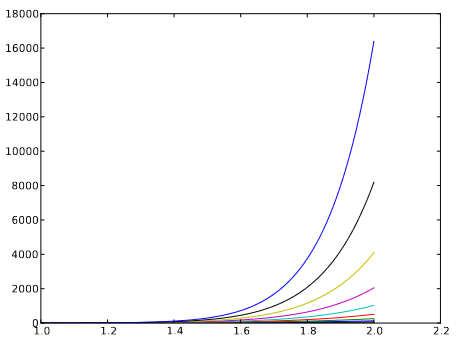
\includegraphics[width=0.7\linewidth]{img_4}
		\caption{The 15 first basis functions $x^{i}, i=0, \ldots, 14$.}
		\label{fig:img_4}
	\end{figure}
	On the other hand, the double precision numpy solver do run for $N=100$, resulting in answers that are not significantly worse than those in the table above, and large powers are associated with small coefficients (e.g., $c_{j}<10^{-2}$ for $10 \leq j \leq 20$ and $c<10^{-5}$ for $\left.j>20\right)$. Even for $N=100$ the approximation still lies on top of the exact curve in a plot (!).
	
	The conclusion is that visual inspection of the quality of the approximation may not uncover fundamental numerical problems with the computations. However, numerical analysts have studied approximations and ill-conditioning for decades, and it is well known that the basis \{1, $x^{2}$, $x^{3}$, \ldots, \} is a bad basis. The best basis from a matrix conditioning point of view is to have orthogonal functions such that $\left(\psi_{i}, \psi_{j}\right)=0$ for $i \neq j$. There are many known sets of orthogonal polynomials and other functions. The functions used in the finite element methods are almost orthogonal, and this property helps to avoid problems with solving matrix systems. Almost orthogonal is helpful, but not enough when it comes to partial differential equations, and ill-conditioning of the coefficient matrix is a theme when solving large-scale matrix systems arising from finite element discretizations.
	\bigbreak
	\section[Fourier series]{Fourier series}
	\label{sec:sec_2_7}
	\noindent A set of sine functions is widely used for approximating functions (the sines are
	also orthogonal as explained more in Section \hyperref[sec:sec_2_6]{2.6}). Let us take
	
	$$
	V=\operatorname{span}\{\sin \pi x, \sin 2 \pi x, \ldots, \sin (N+1) \pi x\}.
	$$
	That is,
	$$
	\psi_{i}(x)=\sin ((i+1) \pi x), \quad i \in \mathcal{I}_{s} .
	$$
	An approximation to the $f(x)$ function from Section \hyperref[sec:sec_2_3]{2.3} can then be computed by the least\textunderscore squares function from Section \hyperref[sec:sec_2_4]{2.4}:
	\begin{lstlisting}[numbers=none]
		N = 3
		from sympy import sin, pi
		x = sp.Symbol('x')
		psi = [sin(pi*(i+1)*x) for i in range(N+1)]
		f = 10*(x-1)**2 - 1
		Omega = [0, 1]
		u, c = least_squares(f, psi, Omega)
		comparison_plot(f, u, Omega)
	\end{lstlisting}
	Figure \hyperref[fig:img_5]{5} (left) shows the oscillatory approximation of $\sum_{j-0}^{N} c_{j} \sin ((j+1) \pi x)$ when $N=3$. Changing $N$ to 11 improves the approximation considerably, see Figure \hyperref[fig:img_5]{5} (right).
	\begin{figure}[H]
		\centering
		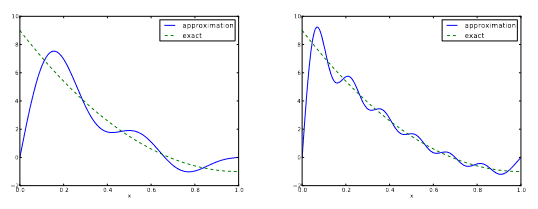
\includegraphics[width=0.7\linewidth]{img_5}
		\caption{Best approximation of a parabola by a sum of 3 (left) and 11 (right) sine functions.}
		\label{fig:img_5}
	\end{figure}
	
	There is an error $f(0)-u(0)=9$ at $x=0$ in Figure \hyperref[fig:img_5]{5} regardless of how large $N$ is, because all $\psi_{i}(0)=0$ and hence $u(0)=0$. We may help the approximation to be correct at $x=0$ by seeking
	\begin{equation}\label{eqa39}
		u(x)=f(0)+\sum_{j \in \mathcal{I}_{s}} c_{j} \psi_{j}(x).
	\end{equation}
	However, this adjustment introduces a new problem at $x=1$ since we now get an error $f(1)-u(1)=f(1)-0=-1$ at this point. A more clever adjustment is to replace the $f(0)$ term by a term that is $f(0)$ at $x=0$ and $f(1)$ at $x=1$. A simple linear combination $f(0)(1-x)+x f(1)$ does the job:
	\begin{equation}\label{eqa40}
		u(x)=f(0)(1-x)+x f(1)+\sum_{j \in \mathcal{I}_{s}} c_{j} \psi_{j}(x).
	\end{equation}
	\noindent This adjustment of $u$ alters the linear system slightly as we get an extra term $-\left(f(0)(1-x)+x f(1), \psi_{i}\right)$ on the right-hand side. Figure \hyperref[fig:img_6]{6} shows the result of this technique for ensuring right boundary values: even 3 sines can now adjust the $f(0)(1-x)+x f(1)$ term such that $u$ approximates the parabola really well, at least visually.
	\begin{figure}[H]
		\centering
		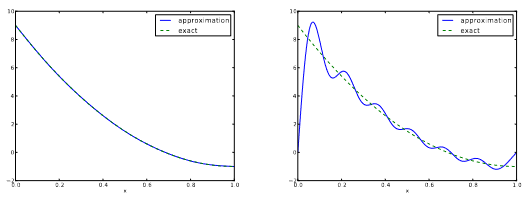
\includegraphics[width=0.7\linewidth]{img_6}
		\caption{Best approximation of a parabola by a sum of 3 (left) and 11 (right)
			sine functions with a boundary term.}
		\label{fig:img_6}
	\end{figure}
	\section[Orthogonal basis functions]{Orthogonal basis functions}
	\label{sec:sec_2_8}
	The choice of sine functions $\psi_{i}(x)=\sin ((i+1) \pi x)$ has a great computational advantage: on $\Omega=[0,1]$ these basis functions are \textit{orthogonal}, implying that $A_{i, j}=0$ if $i \neq j$. This result is realized by trying
	\begin{lstlisting}[numbers=none]
		integrate(sin(j*pi*x)*sin(k*pi*x), x, 0, 1)
	\end{lstlisting}
	in \href{https://www.wolframalpha.com/}{WolframAlpha} (avoid i in the integrand as this symbol means the imaginary unit $\sqrt{-1})$. Also by asking WolframAlpha about $\int_{0}^{1} \sin ^{2}(j \pi x) \mathrm{d} x$, we find it to equal $1 / 2$. With a diagonal matrix we can easily solve for the coefficients by hand:
	\begin{equation}\label{eqa41}
		c_{i}=2 \int_{0}^{1} f(x) \sin ((i+1) \pi x) \mathrm{d} x, \quad i \in \mathcal{I}_{s},
	\end{equation}
	which is nothing but the classical formula for the coefficients of the Fourier sine series of $f(x)$ on $[0,1]$. In fact, when $V$ contains the basic functions used in a Fourier series expansion, the approximation method derived in Section \hyperref[chap:chap_2]{2} results in the classical Fourier series for $f(x)$ (see Exercise \hyperref[sec:sec_10_8]{8} for details).
	
	With orthogonal basis functions we can make the least\textunderscore squares function (much) more efficient since we know that the matrix is diagonal and only the diagonal elements need to be computed:
	\begin{lstlisting}[numbers=none]
		def least_squares_orth(f, psi, Omega):
		N = len(psi) - 1
		A = [0]*(N+1)
		b = [0]*(N+1)
		x = sp.Symbol('x')
		for i in range(N+1):
		A[i] = sp.integrate(psi[i]**2, (x, Omega[0], Omega[1]))
		b[i] = sp.integrate(psi[i]*f, (x, Omega[0], Omega[1]))
		c = [b[i]/A[i] for i in range(len(b))]
		u = 0
		for i in range(len(psi)):
		u += c[i]*psi[i]
		return u, c
	\end{lstlisting}
	This function is found in the file approx1D.py.
	\section[Numerical computations]{Numerical computations}
	\label{sec:sec_2_9}
	\noindent Sometimes the basis functions $\psi_{i}$ and/or the function $f$ have a nature that makes symbolic integration CPU-time consuming or impossible. Even though we implemented a fallback on numerical integration of $\int f \varphi_{i} d x$ considerable time might be required by sympy in the attempt to integrate symbolically. Therefore, it will be handy to have function for fast \textit{numerical} integration and \textit{numerical} solution of the linear system. Below is such a method. It requires Python functions $\mathrm{f}(\mathrm{x})$ and psi $(\mathrm{x}, i)$ for $f(x)$ and $\psi_{i}(x)$ as input. The output is a mesh function with values $u$ on the mesh with points in the array $x$. Three numerical integration methods are offered: scipy. integrate. quad (precision set to $10^{-8}$ ), sympy -mpmath . quad (high precision), and a Trapezoidal rule based on the points in $x$.
	\begin{lstlisting}[numbers=none]
		def least_squares_numerical(f, psi, N, x,
		integration_method='scipy',
		orthogonal_basis=False):
		import scipy.integrate
		A = np.zeros((N+1, N+1))
		b = np.zeros(N+1)
		Omega = [x[0], x[-1]]
		dx = x[1] - x[0]
		
		for i in range(N+1):
		j_limit = i+1 if orthogonal_basis else N+1
		for j in range(i, j_limit):
		print '(%d,%d)' % (i, j)
		if integration_method == 'scipy':
		A_ij = scipy.integrate.quad(
		lambda x: psi(x,i)*psi(x,j),
		Omega[0], Omega[1], epsabs=1E-9, epsrel=1E-9)[0]
		elif integration_method == 'sympy':
		A_ij = sp.mpmath.quad(
		lambda x: psi(x,i)*psi(x,j),
		[Omega[0], Omega[1]])
		else:
		values = psi(x,i)*psi(x,j)
		A_ij = trapezoidal(values, dx)
		A[i,j] = A[j,i] = A_ij
		
		if integration_method == 'scipy':
		b_i = scipy.integrate.quad(			
		lambda x: f(x)*psi(x,i), Omega[0], Omega[1],
		epsabs=1E-9, epsrel=1E-9)[0]
		elif integration_method == 'sympy':
		b_i = sp.mpmath.quad(
		lambda x: f(x)*psi(x,i), [Omega[0], Omega[1]])
		else:
		values = f(x)*psi(x,i)
		b_i = trapezoidal(values, dx)
		b[i] = b_i
		
		c = b/np.diag(A) if orthogonal_basis else np.linalg.solve(A, b)
		u = sum(c[i]*psi(x, i) for i in range(N+1))
		return u, c
		
		def trapezoidal(values, dx):
		"""Integrate values by the Trapezoidal rule (mesh size dx)."""
		return dx*(np.sum(values) - 0.5*values[0] - 0.5*values[-1])
	\end{lstlisting}
	Here is an example on calling the function:
	\begin{lstlisting}[numbers=none]
		from numpy import linspace, tanh, pi
		def psi(x, i):
		return sin((i+1)*x)
		x = linspace(0, 2*pi, 501)
		N = 20
		u, c = least_squares_numerical(lambda x: tanh(x-pi), psi, N, x,
		orthogonal_basis=True)
	\end{lstlisting}
	\section[The interpolation (or collocation) method]{The interpolation (or collocation) method}
	\label{sec:sec_2_10}
	The principle of minimizing the distance between $u$ and $f$ is an intuitive way of computing a best approximation $u \in V$ to $f$. However, there are other approaches as well. One is to demand that $u\left(x_{i}\right)=f\left(x_{i}\right)$ at some selected points $x_{i}, i \in \mathcal{I}_{s}$ :
	\begin{equation}\label{eqa42}
		u\left(x_{i}\right)=\sum_{j \in \mathcal{I}_{s}} c_{j} \psi_{j}\left(x_{i}\right)=f\left(x_{i}\right), \quad i \in \mathcal{I}_{s}.
	\end{equation}
	This criterion also gives a linear system with $N+1$ unknown coefficients
	$\left\{c_{i}\right\}_{i \in \mathcal{I}_{s}}$ :
	\begin{equation}\label{eqa43}
		\sum_{j \in \mathcal{I}_{s}} A_{i, j} c_{j}=b_{i}, \quad i \in \mathcal{I}_{s},
	\end{equation}
	with
	\begin{equation}\label{eqa44}
		A_{i, j} = \psi_{j}\left(x_{i}\right),
	\end{equation}
	\begin{equation}\label{eqa45}
		b_{i} = f\left(x_{i}\right).
	\end{equation}
	This time the coefficient matrix is not symmetric because $\psi_{j}\left(x_{i}\right) \neq \psi_{i}\left(x_{j}\right)$ in general. The method is often referred to as an \textit{interpolation method} since some point values of $f$ are given $\left(f\left(x_{i}\right)\right)$ and we fit a continuous function $u$ that goes through the $f\left(x_{i}\right)$ points. In this case the $x_{i}$ points are called \textit{interpolation points}. When the same approach is used to approximate differential equations, one usually applies the name \textit{collocation method} and $x_{i}$ are known as \textit{collocation points}.
	
	Given $f$ as a sympy symbolic expression $\mathrm{f},\left\{\psi_{i}\right\}_{i \in \mathcal{I}_{s}}$ as a list psi, and a set of points $\left\{x_{i}\right\}_{i \in \mathcal{I}_{s}}$ as a list or array points, the following Python function sets up and solves the matrix system for the coefficients $\left\{c_{i}\right\}_{i \in \mathcal{I}_{s}}$ :
	\begin{lstlisting}[numbers=none]
		def interpolation(f, psi, points):
		N = len(psi) - 1
		A = sp.zeros((N+1, N+1))
		b = sp.zeros((N+1, 1))
		x = sp.Symbol('x')
		# Turn psi and f into Python functions
		psi = [sp.lambdify([x], psi[i]) for i in range(N+1)]
		f = sp.lambdify([x], f)
		for i in range(N+1):
		for j in range(N+1):
		A[i,j] = psi[j](points[i])
		b[i,0] = f(points[i])
		c = A.LUsolve(b)
		u = 0
		for i in range(len(psi)):
		u += c[i,0]*psi[i](x)
		return u	
	\end{lstlisting}	
	The interpolation function is a part of the approx1D module.
	
	We found it convenient in the above function to turn the expressions f
	and psi into ordinary Python functions of x, which can be called with float
	values in the list points when building the matrix and the right-hand side.
	The alternative is to use the subs method to substitute the x variable in an
	expression by an element from the points list. The following session illustrates
	both approaches in a simple setting:\\
	\begin{lstlisting}[numbers=none]
		>>> from sympy import *
		>>> x = Symbol('x')
		>>> e = x**2 # symbolic expression involving x
		>>> p = 0.5 # a value of x
		>>> v = e.subs(x, p) # evaluate e for x=p
		>>> v
		0.250000000000000
		>>> type(v)
		sympy.core.numbers.Float
		>>> e = lambdify([x], e) # make Python function of e
		>>> type(e)
		>>> function
		>>> v = e(p) # evaluate e(x) for x=p
		>>> v
		0.25
		>>> type(v)
		float	
	\end{lstlisting}
	A nice feature of the interpolation or collocation method is that it avoids computing integrals. However, one has to decide on the location of the $x_{i}$ points. A simple, yet common choice, is to distribute them uniformly throughout $\Omega$.
	\bigbreak
	\noindent \textbf{Example.} Let us illustrate the interpolation or collocation method by approximating our parabola $f(x)=10(x-1)^{2}-1$ by a linear function on $\Omega=[1,2]$, using two collocation points $x_{0}=1+1 / 3$ and $x_{1}=1+2 / 3$ :
	\begin{lstlisting}[numbers=none]
		f = 10*(x-1)**2 - 1
		psi = [1, x]
		Omega = [1, 2]
		points = [1 + sp.Rational(1,3), 1 + sp.Rational(2,3)]
		u = interpolation(f, psi, points)
		comparison_plot(f, u, Omega)		
	\end{lstlisting}
	The resulting linear system becomes
	$$
	\left(\begin{array}{ll}
		1 & 4 / 3 \\
		1 & 5 / 3
	\end{array}\right)\left(\begin{array}{l}
		c_{0} \\
		c_{1}
	\end{array}\right)=\left(\begin{array}{l}
		1 / 9 \\
		31 / 9
	\end{array}\right)
	$$
	with solution $c_{0}=-119 / 9$ and $c_{1}=10$. Figure \hyperref[fig:img_7]{7} (left) shows the resulting approximation $u=-119 / 9+10 x$. We can easily test other interpolation points, say $x_{0}=1$ and $x_{1}=2$. This changes the line quite significantly, see Figure \hyperref[fig:img_7]{7} (right).
	\begin{figure}[H]
		\centering
		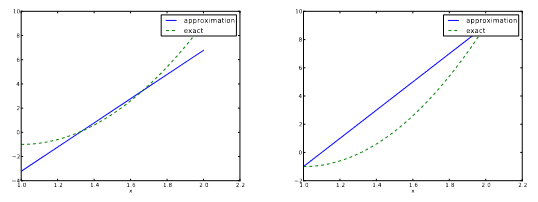
\includegraphics[width=0.7\linewidth]{img_7}
		\caption{Approximation of a parabola by linear functions computed by two
			interpolation points: 4/3 and 5/3 (left) versus 1 and 2 (right).}
		\label{fig:img_7}
	\end{figure}
	\section[Lagrange polynomials]{Lagrange polynomials}
	\label{sec:sec_2_11}
	\noindent In Section \hyperref[sec:sec_2_7]{2.7} we explain the advantage with having a diagonal matrix: formulas for the coefficients $\left\{c_{i}\right\}_{i \in \mathcal{I}_{s}}$ can then be derived by hand. For an interpolation/collocation method a diagonal matrix implies that $\psi_{j}\left(x_{i}\right)=0$ if $i \neq j$. One set of basis functions $\psi_{i}(x)$ with this property is the Lagrange interpolating polynomials, or just \textit{Lagrange polynomials}. (Although the functions are named after Lagrange, they were first discovered by Waring in 1779 , rediscovered by
	Euler in 1783 , and published by Lagrange in 1795.) The Lagrange polynomials have the form
	\begin{equation}\label{eqa46}
		\psi_{i}(x)=\prod_{j=0, j \neq i}^{N} \frac{x-x_{j}}{x_{i}-x_{j}}=\frac{x-x_{0}}{x_{i}-x_{0}} \cdots \frac{x-x_{i-1}}{x_{i}-x_{i-1}} \frac{x-x_{i+1}}{x_{i}-x_{i+1}} \cdots \frac{x-x_{N}}{x_{i}-x_{N}},
	\end{equation}
	for $i \in \mathcal{I}_{s}$. We see from (\hyperref[eqa46]{46}) that all the $\psi_{i}$ functions are polynomials of degree $N$ which have the property
	\begin{equation}\label{eqa47}
		\psi_{i}\left(x_{s}\right)=\delta_{i s}, \quad \delta_{i s}= \begin{cases}1, & i=s, \\ 0, & i \neq s,\end{cases}
	\end{equation}
	when $x_{s}$ is an interpolation/collocation point. Here we have used the \textit{Kronecker delta} symbol $\delta_{i s}$. This property implies that $A_{i, j}=0$ for $i \neq j$ and $A_{i, j}=1$ when $i=j$. The solution of the linear system is them simply
	\begin{equation}\label{eqa48}
		c_{i}=f\left(x_{i}\right), \quad i \in \mathcal{I}_{s},
	\end{equation}
	and
	\begin{equation}\label{eqa49}
		u(x)=\sum_{j \in \mathcal{I}_{s}} f\left(x_{i}\right) \psi_{i}(x).
	\end{equation}
	The following function computes the Lagrange interpolating polynomial $\psi_{i}(x)$, given the interpolation points $x_{0}, \ldots, x_{N}$ in the list or array points:
	\begin{lstlisting}[numbers=none]
		def Lagrange_polynomial(x, i, points):
		p = 1
		for k in range(len(points)):
		if k != i:
		p *= (x - points[k])/(points[i] - points[k])
		return p
	\end{lstlisting}
	The next function computes a complete basis using equidistant points throughout
	$\Omega$:
	\begin{lstlisting}[numbers=none]
		def Lagrange_polynomials_01(x, N):
		if isinstance(x, sp.Symbol):
		h = sp.Rational(1, N-1)
		else:
		h = 1.0/(N-1)
		points = [i*h for i in range(N)]
		psi = [Lagrange_polynomial(x, i, points) for i in range(N)]
		return psi, points	
	\end{lstlisting}
	When $x$ is an sp. Symbol object, we let the spacing between the interpolation points, $\mathrm{h}$, be a sympy rational number for nice end results in the formulas for $\psi_{i}$. The other case, when $\mathrm{x}$ is a plain Python $\mathrm{float}$, signifies numerical computing, and then we let $\mathrm{h}$ be a floating-point number. Observe that the Lagrange\textunderscore polynomial function works equally well in the symbolic and numerical case - just think of x being an sp.Symbol object or a Python float. A little
	interactive session illustrates the difference between symbolic and numerical
	computing of the basis functions and points:
	\begin{lstlisting}[numbers=none]
		>>> import sympy as sp
		>>> x = sp.Symbol('x')
		>>> psi, points = Lagrange_polynomials_01(x, N=3)
		>>> points
		[0, 1/2, 1]
		>>> psi
		[(1 - x)*(1 - 2*x), 2*x*(2 - 2*x), -x*(1 - 2*x)]
		>>> x = 0.5 # numerical computing
		>>> psi, points = Lagrange_polynomials_01(x, N=3)
		>>> points
		[0.0, 0.5, 1.0]
		>>> psi
		[-0.0, 1.0, 0.0]	
	\end{lstlisting}
	The Lagrange polynomials are very much used in finite element methods because
	of their property (\hyperref[eqa47]{47}).
	
	\noindent \textbf{Approximation of a polynomial.} The Galerkin or least squares method lead
	to an exact approximation if f lies in the space spanned by the basis functions. It
	could be interest to see how the interpolation method with Lagrange polynomials
	as basis is able to approximate a polynomial, e.g., a parabola. Running
	\begin{lstlisting}[numbers=none]
		for N in 2, 4, 5, 6, 8, 10, 12:
		f = x**2
		psi, points = Lagrange_polynomials_01(x, N)
		u = interpolation(f, psi, points)	
	\end{lstlisting}
	shows the result that up to $\mathrm{N}=4$ we achieve an exact approximation, and then round-off errors start to grow, such that $\mathrm{N}=15$ leads to a 15 -degree polynomial for $u$ where the coefficients in front of $x^{r}$ for $r>2$ are of size $10^{-5}$ and smaller.
	Successful example. Trying out the Lagrange polynomial basis for approximating $f(x)=\sin 2 \pi x$ on $\Omega=[0,1]$ with the least squares and the interpolation techniques can be done by
	\begin{lstlisting}[numbers=none]
		x = sp.Symbol('x')
		f = sp.sin(2*sp.pi*x)
		psi, points = Lagrange_polynomials_01(x, N)
		Omega=[0, 1]
		u = least_squares(f, psi, Omega)
		comparison_plot(f, u, Omega)
		u = interpolation(f, psi, points)
		comparison_plot(f, u, Omega)	
	\end{lstlisting}
	Figure \hyperref[fig:img_8]{8} shows the results. There is little difference between the least squares and
	the interpolation technique. Increasing \textit{N} gives visually better approximations.
	\begin{figure}[H]
		\centering
		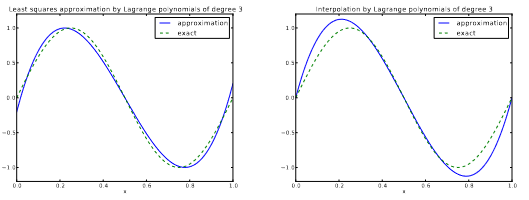
\includegraphics[width=0.7\linewidth]{img_8}
		\caption{Approximation via least squares (left) and interpolation (right) of a
			sine function by Lagrange interpolating polynomials of degree 3.}
		\label{fig:img_8}
	\end{figure}	
	
	\noindent \textbf{Less successful example.} The next example concerns interpolating $f(x)=$ $|1-2 x|$ on $\Omega=[0,1]$ using Lagrange polynomials. Figure \hyperref[fig:img_9]{9} shows a peculiar effect: the approximation starts to oscillate more and more as $N$ grows. This numerical artifact is not surprising when looking at the individual Lagrange polynomials. Figure \hyperref[fig:img_10]{10} shows two such polynomials, $\psi_{2}(x)$ and $\psi_{7}(x)$, both of degree 11 and computed from uniformly spaced points $x_{x_{i}}=i / 11, i=0, \ldots, 11$, marked with circles. We clearly see the property of Lagrange polynomials: $\psi_{2}\left(x_{i}\right)=0$ and $\psi_{7}\left(x_{i}\right)=0$ for all $i$, except $\psi_{2}\left(x_{2}\right)=1$ and $\psi_{7}\left(x_{7}\right)=1$. The most striking feature, however, is the significant oscillation near the boundary. The reason is easy to understand: since we force the functions to zero at so many points, a polynomial of high degree is forced to oscillate between the points. The points, a polynomial of high degree is forced to oscillate between the points. The phenomenon is named Runge's phenomenon and you can read a more detailed explanation on \href{https://en.wikipedia.org/wiki/Runge%27s_phenomenon}{Wikipedia}.
	\bigbreak
	\noindent \textbf{Remedy for strong oscillations.} The oscillations can be reduced by a more clever choice of interpolation points, called the \textit{Chebyshev nodes}:
	\begin{equation}\label{eqa50}
		x_{i}=\frac{1}{2}(a+b)+\frac{1}{2}(b-a) \cos \left(\frac{2 i+1}{2(N+1)} p i\right), \quad i=0 \ldots, N,
	\end{equation}
	on the interval $\Omega=[a, b]$. Here is a flexible version of the Lagrange\textunderscore polynomials\textunderscore 01 function above, valid for any interval $\Omega=[a, b]$ and with the possibility to generate both uniformly distributed points and Chebyshev nodes:
	\begin{lstlisting}[numbers=none]
		def Lagrange_polynomials(x, N, Omega, point_distribution='uniform'):
		if point_distribution == 'uniform':
		if isinstance(x, sp.Symbol):
		h = sp.Rational(Omega[1] - Omega[0], N)
		else:
		h = (Omega[1] - Omega[0])/float(N)
		points = [Omega[0] + i*h for i in range(N+1)]
		elif point_distribution == 'Chebyshev':
		points = Chebyshev_nodes(Omega[0], Omega[1], N)
		psi = [Lagrange_polynomial(x, i, points) for i in range(N+1)]
		return psi, points
		def Chebyshev_nodes(a, b, N):
		from math import cos, pi
		return [0.5*(a+b) + 0.5*(b-a)*cos(float(2*i+1)/(2*N+1))*pi) \
		for i in range(N+1)]
	\end{lstlisting}
	All the functions computing Lagrange polynomials listed above are found in the module file Lagrange.py. Figure 11 shows the improvement of using Chebyshev nodes (compared with Figure \hyperref[fig:img_9]{9}). The reason is that the corresponding Lagrange polynomials have much smaller oscillations as seen in Figure \hyperref[fig:img_12]{12} (compare with Figure \hyperref[fig:img_10]{10}).
	
	Another cure for undesired oscillation of higher-degree interpolating polynomials is to use lower-degree Lagrange polynomials on many small patches of the domain, which is the idea pursued in the finite element method. For instance, linear Lagrange polynomials on $[0,1 / 2]$ and $[1 / 2,1]$ would yield a perfect approximation to $f(x)=|1-2 x|$ on $\Omega=[0,1]$ since $f$ is piecewise linear.
	\begin{figure}[H]
		\centering
		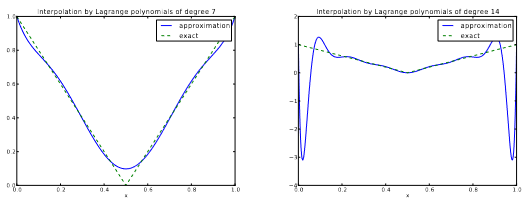
\includegraphics[width=0.7\linewidth]{img_9}
		\caption{Interpolation of an absolute value function by Lagrange polynomials and uniformly distributed interpolation points: degree 7 (left) and 14 (right).}
		\label{fig:img_9}
	\end{figure}
	How does the least squares or projection methods work with Lagrange polynomials? Unfortunately, sympy has problems integrating the $f(x)=|1-2 x|$ function times a polynomial. Other choices of $f(x)$ can also make the symbolic integration fail. Therefore, we should extend the least\textunderscore squares function such that it falls back on numerical integration if the symbolic integration is unsuccessful. In the latter case, the returned value from sympy's integrate function is an object of type Integral. We can test on this type and utilize the mpmath module in sympy to perform numerical integration of high precision. Here is the code:
	\begin{lstlisting}[numbers=none]
		def least_squares(f, psi, Omega):
		N = len(psi) - 1
		A = sp.zeros((N+1, N+1))
		b = sp.zeros((N+1, 1))
		x = sp.Symbol('x')
		for i in range(N+1):
		for j in range(i, N+1):
		integrand = psi[i]*psi[j]
		I = sp.integrate(integrand, (x, Omega[0], Omega[1]))	
	\end{lstlisting}
	\begin{figure}[H]
		\centering
		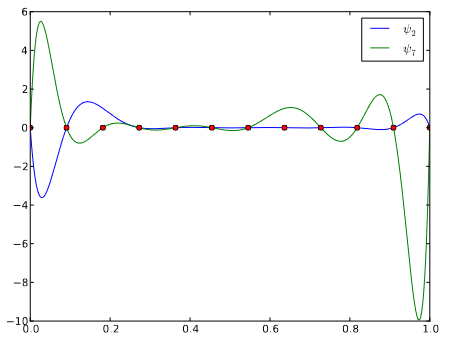
\includegraphics[width=0.7\linewidth]{img_10}
		\caption{Illustration of the oscillatory behavior of two Lagrange polynomials
			based on 12 uniformly spaced points (marked by circles).}
		\label{fig:img_10}
	\end{figure}
	\begin{figure}[H]
		\centering
		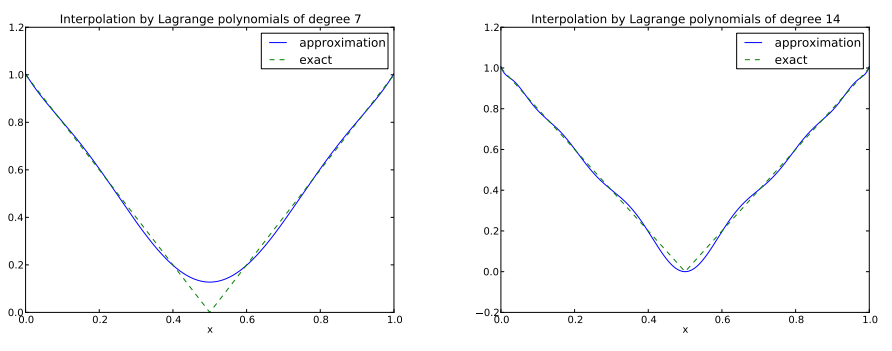
\includegraphics[width=0.7\linewidth]{img_11}
		\caption{ Interpolation of an absolute value function by Lagrange polynomials
			and Chebyshev nodes as interpolation points: degree 7 (left) and 14 (right).}
		\label{fig:img_11}
	\end{figure}
	\begin{lstlisting}[numbers=none]
		if isinstance(I, sp.Integral):
		# Could not integrate symbolically, fallback
		# on numerical integration with mpmath.quad
		integrand = sp.lambdify([x], integrand)
		I = sp.mpmath.quad(integrand, [Omega[0], Omega[1]])
		A[i,j] = A[j,i] = I
		integrand = psi[i]*f
		I = sp.integrate(integrand, (x, Omega[0], Omega[1]))
		if isinstance(I, sp.Integral):
		integrand = sp.lambdify([x], integrand)
	\end{lstlisting}
	\begin{figure}[H]
		\centering
		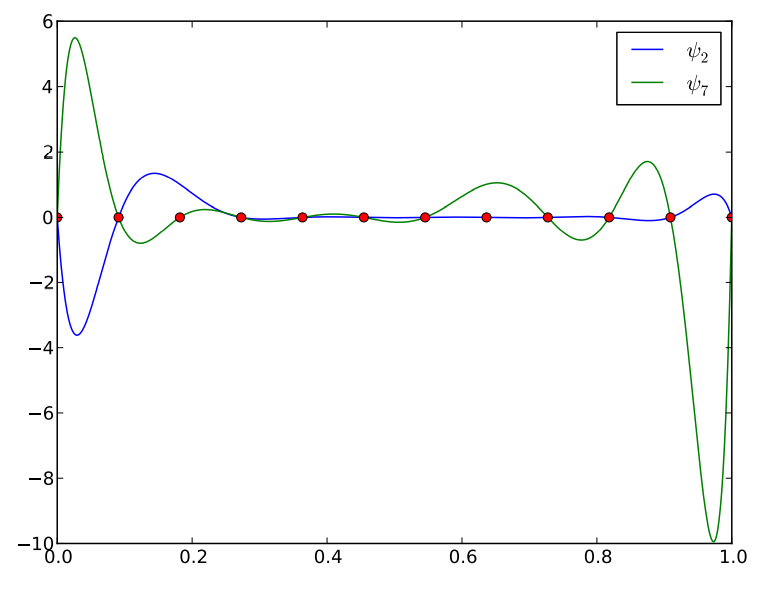
\includegraphics[width=0.7\linewidth]{img_12}
		\caption{Illustration of the less oscillatory behavior of two Lagrange polynomials based on 12 Chebyshev points (marked by circles).}
		\label{fig:img_12}
	\end{figure}
	\begin{lstlisting}[numbers=none]
		I = sp.mpmath.quad(integrand, [Omega[0], Omega[1]])
		b[i,0] = I
		c = A.LUsolve(b)
		u = 0
		for i in range(len(psi)):
		u += c[i,0]*psi[i]
		return u
	\end{lstlisting}
	

\end{document}